\documentclass[14pt]{extarticle}
\usepackage{fontspec}
\usepackage{polyglossia} % use instead of babel
\usepackage{pgfplots}
\usepackage{float}
\usepackage{graphicx}
\usepackage{amsmath}
\usepackage{amsfonts}
\setdefaultlanguage{hebrew}
\setotherlanguage{english}
\newfontfamily\hebrewfont[Script=Hebrew]{Arial}

\usepackage[margin=1in]{geometry}

% Reset equation counter at the start of each section
\usepackage{chngcntr}
\usepackage{etoolbox}
\counterwithin*{equation}{section}
\preto{\section}{\setcounter{equation}{0}}

% Left-aligned equation environment
\newenvironment{lefteqs}{%
    \begin{english}%
    \begin{flushleft}%
    \renewcommand{\arraystretch}{1.3}%
    $\begin{array}{@{}l@{}}%
}{%
    \end{array}$%
    \end{flushleft}%
    \end{english}%
}

\begin{document}

\begin{center}
    {\LARGE \textbf{מעבדה 11}}\\
    {\textbf{ניסוי פרנק הרץ}}
\end{center}

\begin{itemize}
    \item מגישים
    \begin{itemize}
        \item אורי כספי - 331496927
        \item שי רואימי - 318986270
    \end{itemize}
    \item תאריך ביצוע הניסוי: 17 באוגוסט 2026
\end{itemize}

\newpage
\section*{מטרת הניסוי}

\begin{itemize}
    \item מדידת אנרגיה העירור הראשונה של אטום ארגון
    \item חישוב אורך הגל הממוצע הנפלט מגז ארגון כתוצאה מירידת אלקטרונים לרמת היסוד
\end{itemize}

\section*{רקע תיאורטי}

\subsection*{רמות אנרגיה בדידות ופליטת פוטונים}

אלקטרונים באטום אינם יכולים לקבל ערכי אנרגיה רציפים, אלא ערכים בדידים.
הרמה הנמוכה ביותר מכונה רמת היסוד. תוצאה זו נובעת מפתרון משוואת
שרדינגר עבור האלקטרון בשדה הגרעין, המוביל לקוונטיזציה של האנרגיה.

מעבר של אלקטרון בין שתי רמות גורם לבליעה או לפליטה של פוטון בודד. לפוטון אנרגיה התלויה
רק בתדירות (או באורך הגל) של הקרינה:
\begin{equation}
    E = h\nu = \frac{hc}{\lambda}
\end{equation}
כאשר $h$ הקבוע של פלנק, $\nu$ תדירות הקרינה, $\lambda$ אורך הגל ו-$c$ מהירות האור בריק.

משימור אנרגיה, אנרגיית הפוטון הנפלט או הנבלע חייבת להיות שווה בדיוק להפרש האנרגיות בין
שתי הרמות:
\begin{equation}
    h\nu = E_n - E_m
\end{equation}

\subsection*{עירור בהתנגשות אלקטרונים}

אפשרות נוספת לעורר את האטום היא ״להפציץ״ אותו באלקטרונים חופשיים. אלקטרון חופשי הפוגע
באטום יכול להעביר לו חלק מהאנרגיה הקינטית שלו, המתאים בדיוק להפרש בין שתי רמות אנרגיה, ולהמשיך
לנוע עם האנרגיה שנותרה לו. נסמן ב-$E_{12}$ את הפרש האנרגיות בין רמת היסוד לרמה המעוררת
הראשונה - זוהי \textbf{אנרגיית העירור הראשונה} של האטום.

קיימים שני סוגי התנגשויות בין האלקטרון החופשי לאטום:
\begin{itemize}
    \item \textbf{התנגשות אלסטית} - מתרחשת כאשר האנרגיה הקינטית של האלקטרון קטנה מ-$E_{12}$.
    מכיוון שמסת האטום גדולה פי עשרות אלפים ממסת האלקטרון, האלקטרון משנה בעיקר את כיוון תנועתו
    וכמעט אינו מאבד אנרגיה.
    \item \textbf{התנגשות לא אלסטית} - מתרחשת כאשר האנרגיה הקינטית מגיעה ל-$E_{12}$. האלקטרון
    מוסר את האנרגיה לאטום, האטום עולה לרמה המעוררת והאלקטרון נותר כמעט חסר אנרגיה קינטית.
\end{itemize}

\subsection*{שפופרת בניסוי פרנק והרץ}

בשפופרת ישנם קתודה מחוממת $K$ הפולטת אלקטרונים בפליטה תרמיונית, סריג מאיץ $G_2$ שהמתח בינו לבין
הקתודה הוא $V_{G_2K}$, ואנודה $A$ שהפוטנציאל שלה נמוך מזה של הסריג, כך שבין הסריג לאנודה שורר
מתח עצירה $V_{G_2A}$. אלקטרון שעבר את הסריג יגיע לאנודה רק אם האנרגיה הקינטית שלו גדולה
מ-$eV_{G_2A}$, כאשר $e$ מטען האלקטרון.

אלקטרון שנפלט מהקתודה ועבר את מלוא הפרש הפוטנציאלים עד הסריג רוכש אנרגיה קינטית:
\begin{equation}
    E_k = e V_{G_2K}
\end{equation}

כל עוד $E_k < E_{12}$ כל ההתנגשויות אלסטיות, האלקטרונים שומרים על אנרגייתם, ועם הגדלת
$V_{G_2K}$ הזרם באנודה גדל. ברגע ש-$E_k$ משתווה ל-$E_{12}$ מתחילות התנגשויות לא אלסטיות,
האלקטרונים מאבדים אנרגיה ואינם מסוגלים להתגבר על מתח העצירה, והזרם יורד. אם נגדיל את המתח שוב
האלקטרונים יואצו מחדש, \emph{לאחר} ההתנגשות, הזרם יעלה שוב, ובנקודה שבה האנרגיה
שנצברה מחדש שווה שוב ל-$E_{12}$ תתרחש התנגשות לא אלסטית שנייה והזרם ירד שוב. כך מתקבל אופיין
זרם-מתח בעל שיאים החוזרים על עצמם.

מכאן שהמרחק בין שני שיאים סמוכים הוא הפרש הפוטנציאלים שעל האלקטרון לעבור כדי לצבור מחדש
בדיוק את אנרגיית העירור הראשונה:
\begin{equation}
    e \cdot \Delta V = E_{12}
\end{equation}
כאשר $\Delta V = V_{n+1} - V_n$  הוא המרחק בין שני שיאים סמוכים באופיין (גרף זרם כתלות במתח).

אם מודדים את $\Delta V$ בוולטים ואת האנרגיה באלקטרון-וולט, מתקבל הקשר:
\begin{equation}
    E_{12}\,[\mathrm{eV}] = \Delta V\,[\mathrm{V}]
\end{equation}

מ-(4) נובע גם שמיקומם של השיאים תלוי ליניארית במספרם הסידורי:
\begin{equation}
    V_n = \frac{E_{12}}{e} \cdot n + V_0
\end{equation}
כאשר $n$ מספרו הסידורי של השיא, ו-$V_0$ קבוע המכיל את מתח העצירה ואת הפרשי פוטנציאל המגע
בין האלקטרודות. הקבוע $V_0$ אינו משפיע על השיפוע, ולכן שיפוע הישר (6) נותן את אנרגיית העירור
בלי תלות בהיסט קבוע כלשהו של סקאלת המתח.

\subsection*{אורך הגל הנפלט}

האטום המעורר שוהה ברמה המעוררת זמן קצר בלבד, ולאחר מכן חוזר לרמת היסוד תוך פליטת פוטון
שאנרגיתו שווה להפרש הרמות. הצבת $E = E_{12}$ ב-(1) ובידוד אורך הגל נותנת:
\begin{equation}
    \lambda = \frac{hc}{E_{12}}
\end{equation}

\section*{מערכת המדידה ומהלך הניסוי}

השתמשנו במערכת פרנק והרץ בנוייה מראש הכוללת שפופרת מלאה בגז ארגון. בניגוד לניסוי המקורי,
שנערך באדי כספית והצריך חימום השפופרת לכ-$180^\circ C$ לצורך קבלת צפיפות אדים מתאימה,
הארגון הוא גז בטמפרטורת החדר ולכן לא נדרש חימום כלל.

השפופרת שבמערכת מכילה שני סריגים ולא אחד. הסריג הנוסף, $G_1$, נמצא בסמוך לקתודה ומוחזק
בפוטנציאל שלילי ביחס אליה. ליד הקתודה מצטבר מטען מרחבי של אלקטרונים שנפלטו, וההתנגשויות
ביניהם יוצרות התפלגות רחבה של אנרגיות. הפוטנציאל השלילי על $G_1$ מאפשר רק לאלקטרונים
שאנרגיתם הקינטית גבוהה מסף מסוים לעבור אל התווך שבין $G_1$ ל-$G_2$, ובכך מצמצם את התפלגות
האנרגיות ויוצר שיאים חדים יותר בגרף (האופיין).

בפאנל השליטה במערכת יש שלושה פוטנציומטרים נפרדים לשליטה במתחים, מד מתח אנלוגי עם בורר ושלוש סקאלות
($V_{G_1K}$ בתחום $1.3-5V$, $V_{G_2A}$ בתחום $10-15V$, $V_{G_2K}$ בתחום $0-100V$), ומד זרם
אנלוגי עם בורר תחום רגישות. הקריאה במד הזרם מוכפלת בפקטור הרגישות שנבחר כדי לקבל את הזרם
בין $G_2$ לאנודה.

\subsection*{חלק ראשון - מדידה ידנית}

לפני הדלקת המערכת סובבנו את פוטנציומטר $V_{G_2K}$ נגד כיוון השעון עד הסוף. הצבנו את בורר
המדידה במצב ידני, את בורר מתח ההסקה על $V_H = 4V$ ואת בורר תחום הרגישות על $10^{-8}$.

לאחר הדלקת המכשיר כיוונו את המתחים באמצעות בורר מד המתח והפוטנציומטרים המתאימים:
$V_{G_1K} = 2.5V$ ו-$V_{G_2A} = 9V$. לאחר מכן אפסנו את $V_{G_2K}$ וודאנו שמד הזרם מצביע על 0.

העלינו את $V_{G_2K}$ בקפיצות של $2V$ עד $80V$ - ובדקנו בכל שלב את
קריאת מד הזרם. את המדידות השתדלנו לבצע ברצף מבלי לחכות להתייצבות המחט, בגלל הסיכוי לסחיפה של הזרם הנמדד.

לאחר סיום המדידות הצבנו את מתח ההסקה על $4.5V$, שינינו את תחום הרגישות ל-$10^{-7}$
וחזרנו על אותה סדרת מדידות.

\subsection*{חלק שני - מדידה באוסילוסקופ}

חיברנו למערכת אוסילוסקופ. את יציאת $X$
של המערכת לכניסת $X$ של האוסילוסקופ ואת יציאת $Y$ לכניסת $Y$, שתיהן ביחס ליציאת ההארקה.
יציאת $X$ מספקת מתח פרופורציוני למתח ההאצה ויציאת $Y$ מתח פרופורציוני לזרם האלקטרונים.

הצבנו את מתח ההסקה על $4V$, העברנו את בורר המדידה למצב אוטומטי וסובבנו את פוטנציומטר
הסריקה למקסימום. במצב זה מתח ההאצה נסרק מחזורית מאפס עד לערך המרבי שנקבע בפוטנציומטר הסריקה.

הדלקנו את האוסילוסקופ, כיוונו אותו למצב $XY$ וכיוונו את סקאלות המתח בשני הצירים עד לקבלת
תמונה ברורה על הצג. הסקאלה האופקית שנבחרה הייתה $5.00V$ לשנתה והאנכית $20.0mV$ לשנתה.
צילמנו את צג האוסילוסקופ ומדדנו על גבי הסקאלה את המרחקים האופקיים בין השיאים.

\section*{תוצאות וניתוח}

\subsection*{חלק ראשון - אופייני השפופרת}

הטבלה שלהלן מרכזת את קריאות מד הזרם כפונקציה של מתח ההאצה $V_{G_2K}$, עבור שני מתחי ההסקה.
נזכיר כי הזרם מתקבל מהכפלת הקריאה בפקטור הרגישות, שהיה $10^{-8}$ במדידה הראשונה
ו-$10^{-7}$ בשנייה. פקטור זה הוא מכפלה בקבוע ולכן אינו משפיע כלל על מיקומי השיאים, שהם
הגודל היחיד שממנו נגזרת התוצאה.

\begin{table}[H]
    \centering
    \renewcommand{\arraystretch}{1.3}
    \begin{tabular}{|c|c|c||c|c|c|}
        \hline
        \text{[V] $V_{G_2K}$} & \text{$4.0V$ [mA]} & \text{$4.5V$ [mA]} &
        \text{[V] $V_{G_2K}$} & \text{$4.0V$ [mA]} & \text{$4.5V$ [mA]} \\ \hline
        0 & 0.115 & 0.12 & 42 & 0.26 & 0.2 \\ \hline
        2 & 0.117 & 0.12 & 44 & 0.18 & 0.16 \\ \hline
        4 & 0.118 & 0.12 & 46 & 0.14 & 0.14 \\ \hline
        6 & 0.119 & 0.12 & 48 & 0.155 & 0.14 \\ \hline
        8 & 0.119 & 0.12 & 50 & 0.24 & 0.18 \\ \hline
        10 & 0.12 & 0.12 & 52 & 0.31 & 0.22 \\ \hline
        12 & 0.12 & 0.125 & 54 & 0.3 & 0.22 \\ \hline
        14 & 0.14 & 0.14 & 56 & 0.24 & 0.19 \\ \hline
        16 & 0.17 & 0.15 & 58 & 0.18 & 0.16 \\ \hline
        18 & 0.18 & 0.16 & 60 & 0.17 & 0.15 \\ \hline
        20 & 0.16 & 0.14 & 62 & 0.21 & 0.16 \\ \hline
        22 & 0.138 & 0.13 & 64 & 0.28 & 0.2 \\ \hline
        24 & 0.125 & 0.13 & 66 & 0.325 & 0.23 \\ \hline
        26 & 0.165 & 0.15 & 68 & 0.32 & 0.23 \\ \hline
        28 & 0.225 & 0.18 & 70 & 0.27 & 0.2 \\ \hline
        30 & 0.22 & 0.18 & 72 & 0.22 & 0.18 \\ \hline
        32 & 0.17 & 0.15 & 74 & 0.24 & 0.18 \\ \hline
        34 & 0.13 & 0.13 & 76 & 0.3 & 0.21 \\ \hline
        36 & 0.13 & 0.14 & 78 & 0.36 & 0.24 \\ \hline
        38 & 0.22 & 0.18 & 80 & 0.36 & 0.24 \\ \hline
        40 & 0.28 & 0.21 &  & &  \\ \hline
    \end{tabular}
    \caption{קריאות מד הזרם כפונקציה של מתח ההאצה, עבור מתחי הסקה $4.0V$ ו-$4.5V$}
    \label{tab:l11_manual}
\end{table}

\begin{figure}[H]
    \centering
    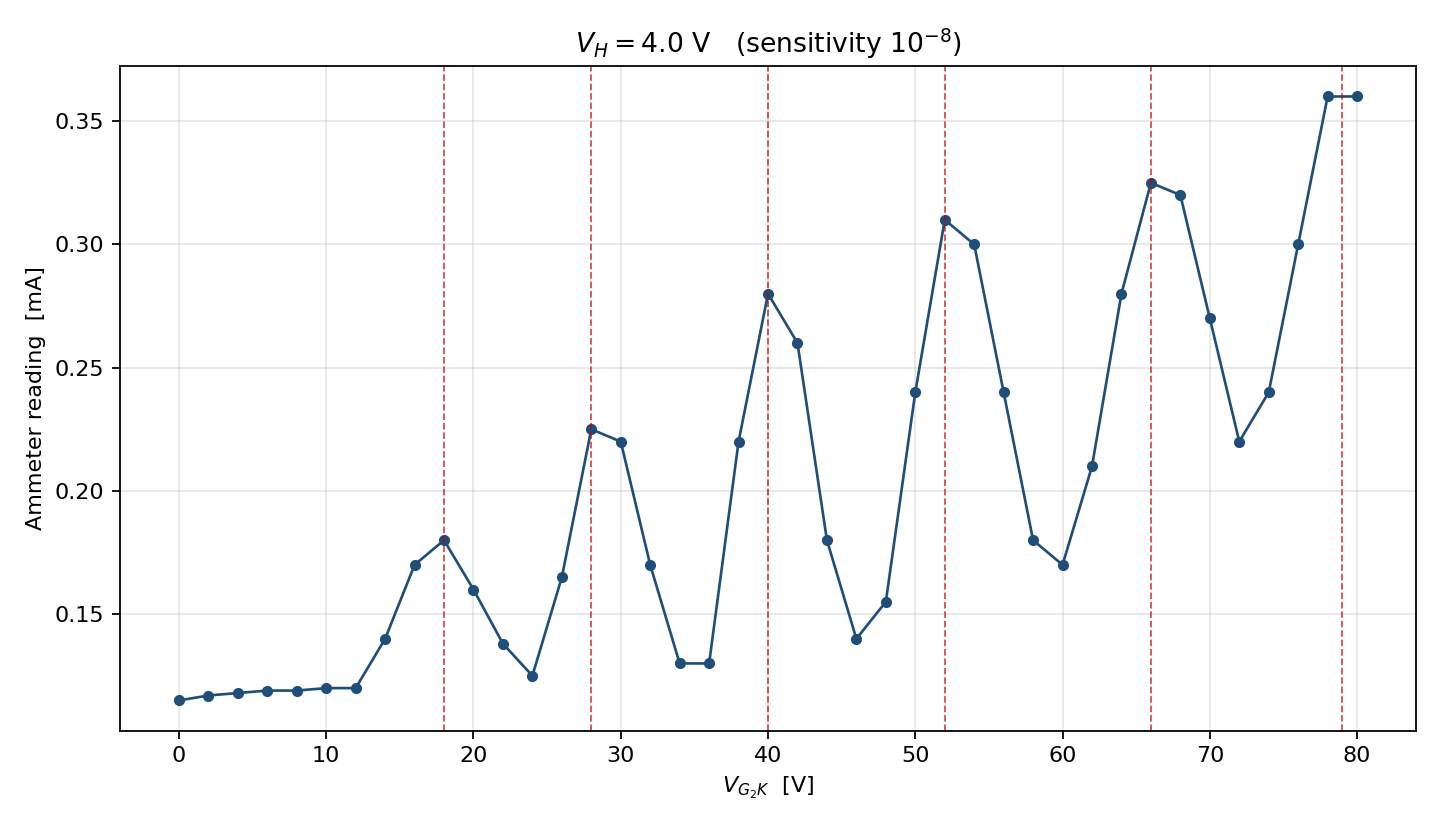
\includegraphics[width=0.9\textwidth]{L11E1_graph.png}
    \caption{אופיין השפופרת עבור מתח הסקה $4.0V$. הקווים המקווקווים מסמנים את מיקומי השיאים}
\end{figure}

\begin{figure}[H]
    \centering
    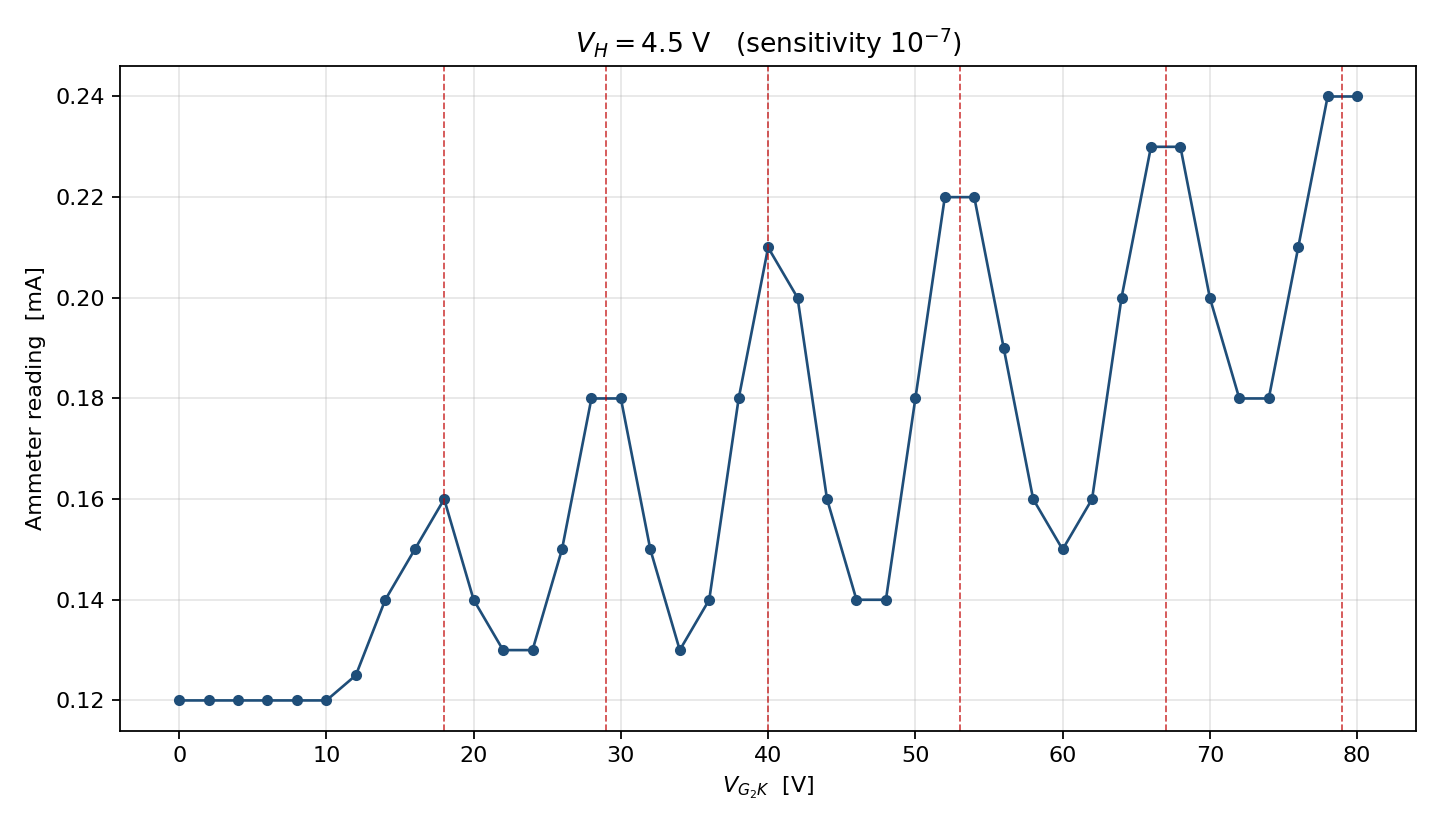
\includegraphics[width=0.9\textwidth]{L11E2_graph.png}
    \caption{אופיין השפופרת עבור מתח הסקה $4.5V$. הקווים המקווקווים מסמנים את מיקומי השיאים}
\end{figure}

בשני האופיינים מתקבלת אותה תמונה איכותית: הזרם כמעט קבוע עד $V_{G_2K} \approx 12V$, ומשם ואילך
מופיעה סדרה של שישה שיאים וביניהם נקודות מינימום מקומיות, כאשר ישנה מגמת עלייה בזרם בין כל שיא.

הקריאה במתח אפס אינה אפס אלא כ-$0.12mA$. סוגייה זו מתוארת גם בהוראות הניסוי בתור תקלה במד הזרם.
מכיוון שהניתוח מקוסס על מיקומי השיאים בציר המתח ולא על ערכי הזרם, תקלה זו לא משפיעה על התוצאה.

תחילת העלייה בזרם סביב $V_{G_2K} \approx 12V$ עקבית עם מבנה מערכת הניסוי. אלקטרון שמגיע לסריג
$G_2$ צריך אנרגיה קינטית הגדולה מ-$eV_{G_2A} = 9\,eV$ כדי להתגבר על מתח העצירה ולהגיע לאנודה,
ולכן מתחת לסף זה כמעט שאין זרם באנודה.

\subsubsection*{מיקומי השיאים והמרחקים ביניהם}

מדידת המתח בוצעה בקפיצות של $2V$, ולכן מיקום שיא נקבע לפי המתח שבו התקבלה הקריאה המרבית.
כאשר שתי נקודות סמוכות נתנו את אותה קריאת מקסימום מקומי לקחנו את ממוצע הערכים.

הטבלה מכילה את ערכי המתח עבורם מתקבל שיא בזרם, ואת הפרשי המתחים בין השיאים:

\begin{table}[H]
    \centering
    \renewcommand{\arraystretch}{1.5}
    \begin{tabular}{|c|c|c|c|c|}
        \hline
        \text{$n$} & \text{[V] $4.0V$ - $V_n$} & \text{[V] $\Delta V$} &
        \text{[V] $4.5V$ - $V_n$} & \text{[V] $\Delta V$} \\ \hline
        1 & 18 & --- & 18 & --- \\ \hline
        2 & 28 & 10 & 29 & 11 \\ \hline
        3 & 40 & 12 & 40 & 11 \\ \hline
        4 & 52 & 12 & 53 & 13 \\ \hline
        5 & 66 & 14 & 67 & 14 \\ \hline
        6 & 79 & 13 & 79 & 12 \\ \hline
    \end{tabular}
    \caption{מיקומי השיאים באופיין והמרחקים בין שיאים סמוכים}
    \label{tab:l11_peaks}
\end{table}

\subsubsection*{אנרגיית העירור - מתח הסקה $4.0V$}

הערך הטוב ביותר עבור המרחק בין שיאים סמוכים הוא הממוצע החשבוני של חמשת ההפרשים:
\begin{lefteqs}
    \Delta V = \frac{1}{N}\sum_{i=1}^{N} \Delta V_i
    = \frac{10 + 12 + 12 + 14 + 13}{5} = 12.2\,V
\end{lefteqs}

חמשת ההפרשים הם חמש מדידות בלתי תלויות של אותו גודל, ולכן הפיזור ביניהם מייצג את
אי-הוודאות האקראית. לפי נוסחה (2) בפרק השגיאות:
\begin{lefteqs}
    \Delta_s (\Delta V) = \sqrt{\frac{\sum_{i=1}^{N}\left(\Delta V_i - \Delta V\right)^2}{N}} \\
    \Delta_s (\Delta V) = \sqrt{\frac{(-2.2)^2 + (-0.2)^2 + (-0.2)^2 + 1.8^2 + 0.8^2}{5}}
    = \sqrt{\frac{8.8}{5}} = 1.33\,V
\end{lefteqs}

לגבי שגיאת המכשיר: את מתח ההאצה כיוונו וקראנו במד המתח בקפיצות של $2V$, ולכן הרזולוציה שבה
אנו מסוגלים למקם שיא היא מחצית הצעד:
\begin{lefteqs}
    \Delta_m V = 1\,V
\end{lefteqs}

נשים לב כי ממוצע ההפרשים הוא סכום טלסקופי:
\begin{lefteqs}
    \overline{\Delta V} = \frac{1}{N}\sum_{i=1}^{N}\left(V_{i+1} - V_i\right) = \frac{V_6 - V_1}{N}
\end{lefteqs}
כלומר מיקומי השיאים הפנימיים מצטמצמים, והממוצע תלוי רק בשיא הראשון ובשיא האחרון. לכן שגיאת
המכשיר של הממוצע היא סכום שתי שגיאות המיקום בלבד, מחולק במספר ההפרשים:
\begin{lefteqs}
    \Delta_m (\overline{\Delta V}) = \frac{\Delta_m V + \Delta_m V}{N} = \frac{1 + 1}{5} = 0.4\,V
\end{lefteqs}

השגיאה הכוללת מתקבלת מנוסחה (4) בפרק השגיאות:
\begin{lefteqs}
    \Delta(\overline{\Delta V}) = \sqrt{\left(\Delta_m(\overline{\Delta V})\right)^2 + \left(\Delta_s(\Delta V)\right)^2}
    = \sqrt{0.4^2 + 1.33^2} = 1.39\,V
\end{lefteqs}

לפי (5), אנרגיית העירור הראשונה של אטום הארגון היא:
\begin{lefteqs}
    E_{12} = 12.2 \pm 1.4\,eV
\end{lefteqs}

\subsubsection*{אנרגיית העירור - מתח הסקה $4.5V$}

באותו אופן, עבור מתח הסקה $4.5V$:
\begin{lefteqs}
    \overline{\Delta V} = \frac{11 + 11 + 13 + 14 + 12}{5} = 12.2\,V
\end{lefteqs}
\begin{lefteqs}
    \Delta_s (\Delta V) = \sqrt{\frac{(-1.2)^2 + (-1.2)^2 + 0.8^2 + 1.8^2 + (-0.2)^2}{5}}
    = \sqrt{\frac{6.8}{5}} = 1.17\,V
\end{lefteqs}
שגיאת המכשיר זהה, כיוון ואותה מערכת ואותן קפיצות במתח נעשו גם כאן:
\begin{lefteqs}
    \Delta_m (\overline{\Delta V}) = \frac{1 + 1}{5} = 0.4\,V
\end{lefteqs}
\begin{lefteqs}
    \Delta(\overline{\Delta V}) = \sqrt{0.4^2 + 1.17^2} = 1.23\,V
\end{lefteqs}

ולכן:
\begin{lefteqs}
    E_{12} = 12.2 \pm 1.2\,eV
\end{lefteqs}

שתי המדידות נתנו ערך מרכזי זהה. מכיוון ששתיהן בוצעו באותה מערכת ובאותה שיטה, איננו מתייחסים
אליהן כאל מדידות בלתי תלויות לחלוטין, ולכן נבחר את
השגיאה הגדולה מבין השתיים (בחירה פסימית ובטוחה יותר):
\begin{lefteqs}
    E_{12}^{\text{ידנית}} = 12.2 \pm 1.4\,eV
\end{lefteqs}

\subsubsection*{דרך נוספת להערכת שגיאת המדידה - רגרסיה ליניארית}

הערכת השגיאה שלעיל מתבססת רק על הפיזור בין חמישה הפרשים, ולכן היא רגישה לשגיאה במיקומו
של שיא אחד. דרך נוספת ובלתי תלויה להעריך את שגיאת המדידה היא להשתמש ב-(6): מיקומי השיאים
צריכים להיות פונקציה ליניארית של המספר הסידורי $n$, כאשר השיפוע הוא $E_{12}/e$. התאמת ישר
לכל שישה מיקומי השיאים מנצלת את כל המידע שבמדידה ולא רק את שני קצותיה.

את שגיאות ההתאמה חישבנו לפי נוסחה (17) בפרק השגיאות:
\begin{lefteqs}
    \Delta y = \sqrt{\frac{1}{N-2}\sum\left(y_i - a x_i - b\right)^2} \\
    \Delta a = \Delta y \sqrt{\frac{N}{A}} \,, \quad
    \Delta b = \Delta y \sqrt{\frac{S_{xx}}{A}} \\
    A = N S_{xx} - S_x^2 \,, \quad S_{xx} = \sum x_i^2 \,, \quad S_x = \sum x_i
\end{lefteqs}
כאשר $x_i = n$, $y_i = V_n$, ו-$N = 6$ מספר השיאים. החישוב בוצע באמצעות פונקציית
\begin{english}LINEST\end{english} באקסל, המיישמת נוסחאות אלו.

עבור מתח הסקה $4.0V$:
\begin{lefteqs}
    a = 12.31\,V \,, \quad \Delta a = 0.32\,V \,, \quad b = 4.07\,V \,, \quad \Delta b = 1.24\,V \,, \quad R^2 = 0.9973
\end{lefteqs}
ועבור מתח הסקה $4.5V$:
\begin{lefteqs}
    a = 12.34\,V \,, \quad \Delta a = 0.27\,V \,, \quad b = 4.47\,V \,, \quad \Delta b = 1.07\,V \,, \quad R^2 = 0.9980
\end{lefteqs}

כלומר, בעיגול בהתאם לגודל השגיאה:
\begin{lefteqs}
    E_{12} = 12.3 \pm 0.3\,eV \quad (V_H = 4.0V) \\
    E_{12} = 12.3 \pm 0.3\,eV \quad (V_H = 4.5V)
\end{lefteqs}

השיפועים מסכימים עם ממוצע ההפרשים בתוך שגיאה אחת, אך השגיאה קטנה פי ארבע בערך. ההסבר הוא
שממוצע ההפרשים מסתמך רק על השיא הראשון והאחרון, ואילו ההתאמה משתמשת בכל שש השיאים ומצמצמת
בכך את השפעת שגיאת המיקום של שיא יחיד.

\subsection*{חלק שני - מדידה באוסילוסקופ}

\begin{figure}[H]
    \centering
    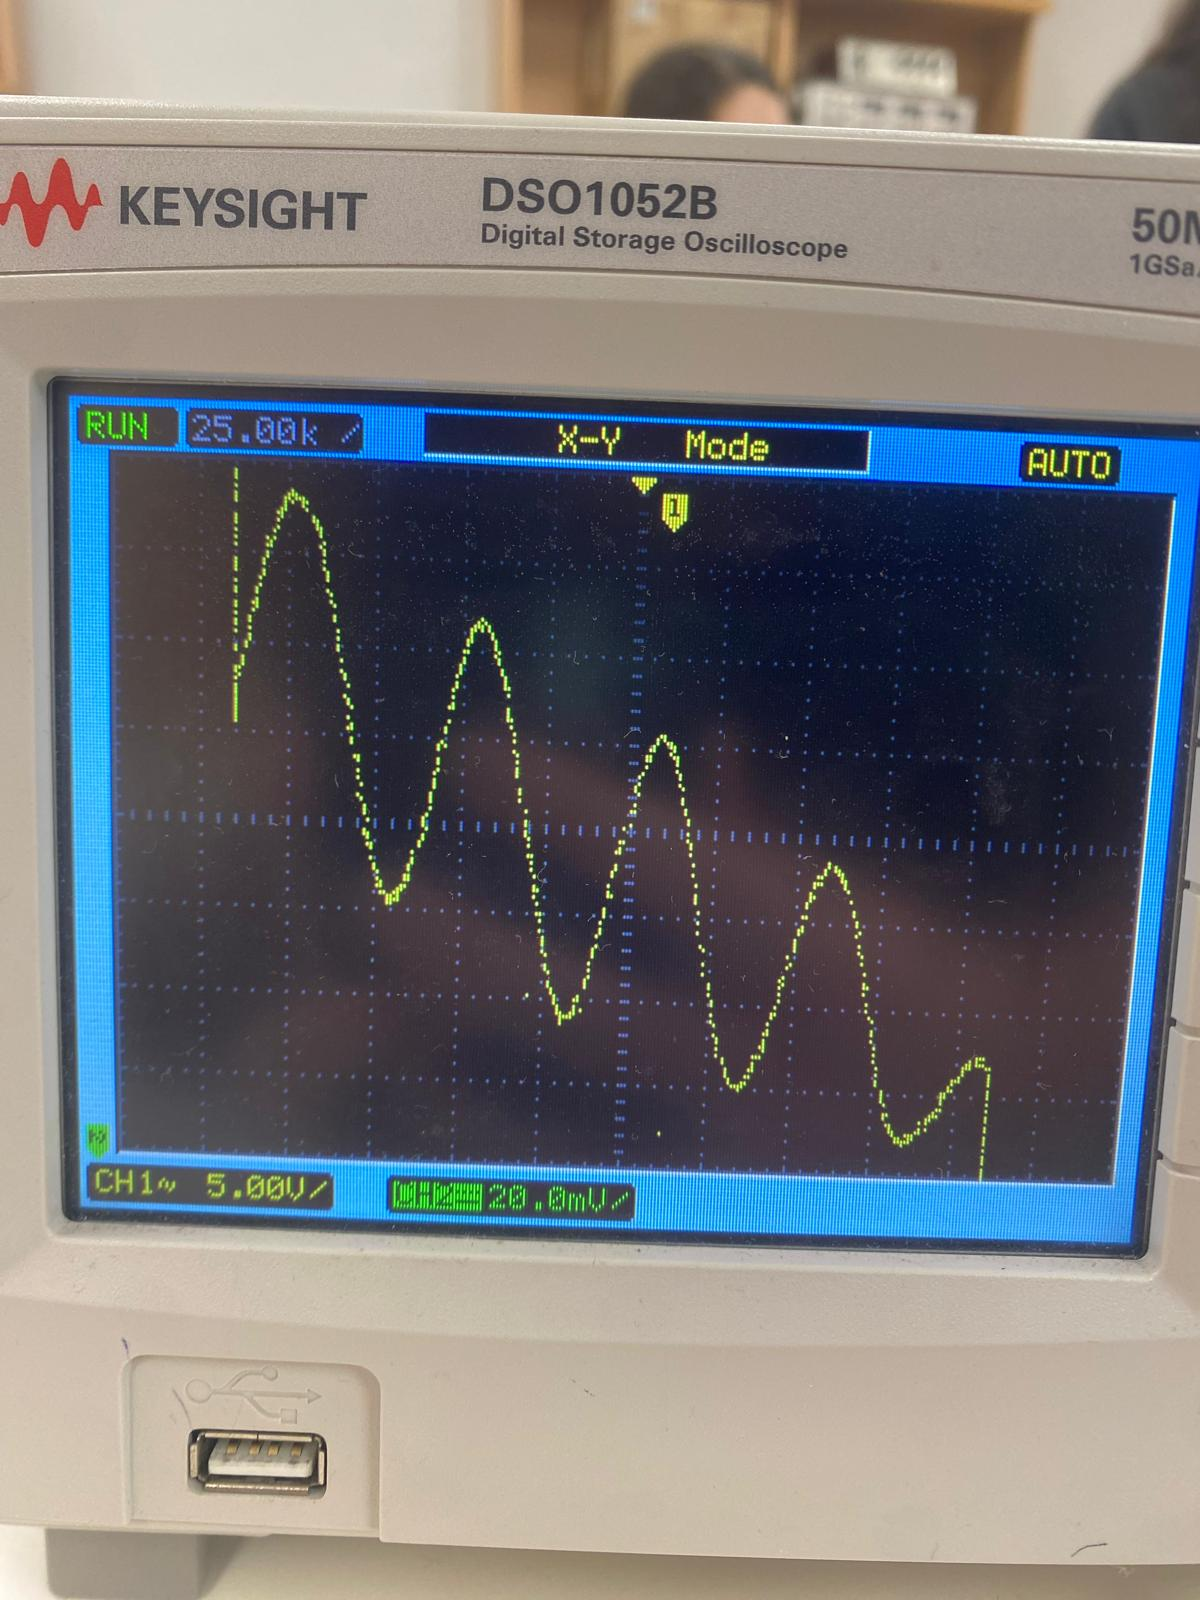
\includegraphics[width=0.75\textwidth]{osciloscope_image.jpg}
    \caption{אופיין השפופרת כפי שהתקבל על צג האוסילוסקופ}
\end{figure}

על הצג ניתן לזהות ארבעה שיאים. השיא החמישי נחתך בקצה הימני לא כללנו אותו במדידה. מדדנו את המרחקים האופקיים בין השיאים על גבי הסקאלה, בדיוק של
$0.1$ שנתה, והמרנו לוולטים לפי הסקאלה האופקית $5.00V$ לשנתה:

\begin{table}[H]
    \centering
    \renewcommand{\arraystretch}{1.5}
    \begin{tabular}{|c|c|c|}
        \hline
        \text{זוג שיאים} & \text{[שנתות] מרחק} & \text{[V] $\Delta V$} \\ \hline
        $1 \rightarrow 2$ & 2.2 & 11.0 \\ \hline
        $2 \rightarrow 3$ & 2.1 & 10.5 \\ \hline
        $3 \rightarrow 4$ & 2.0 & 10.0 \\ \hline
    \end{tabular}
    \caption{המרחקים בין שיאים סמוכים כפי שנמדדו על צג האוסילוסקופ}
    \label{tab:l11_scope}
\end{table}

הממוצע:
\begin{lefteqs}
    \overline{\Delta V} = \frac{11.0 + 10.5 + 10.0}{3} = 10.5\,V
\end{lefteqs}

השגיאה הסטטיסטית לפי נוסחה (2) בפרק השגיאות:
\begin{lefteqs}
    \Delta_s (\Delta V) = \sqrt{\frac{0.5^2 + 0^2 + (-0.5)^2}{3}} = \sqrt{\frac{0.5}{3}} = 0.41\,V
\end{lefteqs}

שגיאת המדידה נובעת מדיוק קריאת מיקום השיא על גבי הסקאלה, $0.1$ שנתה, כלומר $0.5V$ לכל שיא.
גם כאן הממוצע הוא סכום טלסקופי, $\overline{\Delta V} = (V_4 - V_1)/3$, ולכן:
\begin{lefteqs}
    \Delta_m (\overline{\Delta V}) = \frac{0.5 + 0.5}{3} = 0.33\,V
\end{lefteqs}

השגיאה הכוללת:
\begin{lefteqs}
    \Delta(\overline{\Delta V}) = \sqrt{0.33^2 + 0.41^2} = 0.53\,V
\end{lefteqs}

ולכן, לפי (5):
\begin{lefteqs}
    E_{12}^{\text{אוסילוסקופ}} = 10.5 \pm 0.5\,eV
\end{lefteqs}

\subsection*{אורך הגל הנפלט}

את אורך הגל נחשב לפי (7) מתוך תוצאת המדידה הידנית, שהיא המדידה הטובה יותר
(התייחסנו לזה בפרק דיון ומסקנות של הדוח):
\begin{lefteqs}
    \lambda = \frac{hc}{E_{12}} = \frac{6.626 \cdot 10^{-34} \cdot 2.998 \cdot 10^{8}}{12.2 \cdot 1.602 \cdot 10^{-19}}
    = 1.016 \cdot 10^{-7}\,m = 102\,nm
\end{lefteqs}

$\lambda$ היא פונקציה של גודל נמדד יחיד, $E_{12}$, ולכן נשתמש בשיטת הדיפרנציאל (נוסחה (11)
בפרק השגיאות):
\begin{lefteqs}
    \Delta \lambda = \left| \frac{d\lambda}{dE_{12}} \right| \Delta E_{12}
    = \frac{hc}{E_{12}^2} \Delta E_{12} = \lambda \cdot \frac{\Delta E_{12}}{E_{12}}
\end{lefteqs}
כלומר השגיאה היחסית באורך הגל שווה לשגיאה היחסית באנרגיה. נציב:
\begin{lefteqs}
    \Delta \lambda = 102 \cdot \frac{1.4}{12.2} = 11.7\,nm
\end{lefteqs}

התוצאה הסופית:
\begin{lefteqs}
    \lambda = 102 \pm 12\,nm
\end{lefteqs}

\section*{דיון ומסקנות}

סיכום התוצאות שקיבלנו:
\begin{lefteqs}
    E_{12}^{\text{ידנית}} = 12.2 \pm 1.4\,eV \\
    E_{12}^{\text{ידנית, רגרסיה}} = 12.3 \pm 0.3\,eV \\
    E_{12}^{\text{אוסילוסקופ}} = 10.5 \pm 0.5\,eV \\
    \lambda = 102 \pm 12\,nm
\end{lefteqs}

התוצאה המרכזית של הניסוי היא לא מספרים בודדים, אלא צורת האופיין.
אם כל ההתנגשויות בין האלקטרונים לאטומי הארגון היו אלסטיות הזרם היה עולה מונוטונית עם מנת ההאצה,
אבל בפועל התקבלו בשתי האופיינים סדרה של שיאים במרחקים שווים בקירוב
(כנ"ל גם בתוצאה באוסילוקסופ).

המבנה המחזורי הזה של שיאים הוא זה שמצביע על זה שקיימות רמות אנרגיה דסקרטיות שהאטום מסוגל לקלוט.

הטענה שמיקומי השיאים מקיימים את (6) נבדקה כמותית באמצעות ההתאמה הליניארית: התקבלו
$R^2 = 0.9973$ ו-$R^2 = 0.9980$ עבור שני מתחי ההסקה, והשאריות המרביות היו בסדר גודל של
$1.5V$.

אנרגיית העירור הראשונה של אטום הארגון הידועה מן הספרות היא $E_{12} = 11.55\,eV$.
הסטיות היחסיות הן:
\begin{lefteqs}
    \frac{\left| 12.2 - 11.55 \right|}{11.55} = 0.056 \approx 5.6\%  \\
    \frac{\left| 12.3 - 11.55 \right|}{11.55} = 0.068 \approx 6.8\%  \\
    \frac{\left| 10.5 - 11.55 \right|}{11.55} = 0.091 \approx 9.1\% 
\end{lefteqs}

הערך הידוע נמצא בתוך טווח השגיאה של המדידה הידנית, $[10.8, 13.6]\,eV$, ולכן המדידה
הידנית מסכימה עם הערך המקובל. השגיאה היחסית בתוצאה זו היא $11\%$, קטנה מהסף המקובל של
$20\%-25\%$, ולכן התוצאה משמעותית.

תוצאת האוסילוסקופ, $10.5 \pm 0.5\,eV$, נמוכה מהערך הידוע ואינה מכילה אותו בטווח השגיאה
$[10.0, 11.0]\,eV$.

\subsection*{השוואה בין שתי שיטות המדידה}

המדידה הידנית נתנה ערכים קרובים יותר לערך שבספרות מאשר המדידה באוסילוסקופ, גם במרחק המוחלט
מהערך הידוע וגם בכך שהיא מסכימה איתו בתוך טווח השגיאה.

ראשית, במדידה הידנית ציר המתח הוא מד המתח של המערכת עצמה, הנקרא ישירות בוולטים. במדידה
באוסילוסקופ ציר המתח האופקי הוא סקאלת המכשיר, ואנו מניחים שהמתח ביציאת $X$ שווה בדיוק למתח
ההאצה. הנחה זו לא נבדקה בניסוי אל מול קריאת מד המתח שבפאנל המכשיר. עדות לכך שקיימת בעיה בציר האופקי היא שהמרחקים בין השיאים
שנמדדו על הצג יורדים באופן מונוטוני ($11.0$, $10.5$, $10.0$ וולט), אף על פי שלפי (4) הם אמורים
להיות שווים.

שנית, טווח המדידה קטן יותר. במדידה הידנית סרקנו את המתח עד $80V$ וזיהינו שישה שיאים,
כלומר חמישה הפרשים. על הצג של האוסילוסקופ ניתן היה למקם ארבעה שיאים בלבד, כלומר שלושה הפרשים. מספר קטן
יותר של הפרשים גורם לממוצע להיות רגיש יותר לשגיאה במיקומו של שיא יחיד.

שלישית, רזולוציית המדידה. על הצג ניתן לקרוא מיקום שיא בדיוק של כ-$0.1$ שנתה, שהם $0.5V$,
ואילו במדידה הידנית מיקום השיא נקבע בדיוק של $1V$.

\subsection*{תפקידו של מתח ההסקה}

מתח ההסקה שולט על הזרם העובר בגוף החימום של הקתודה ולכן על הטמפרטורה. ככל שהטמפרטורה גבוהה
יותר, כך גדל שטף האלקטרונים הנפלטים מהקתודה בפליטה תרמיונית. ולכן השפעות על האופיין היא על
\emph{סקאלת הזרם} בלבד, ולא על מיקומי השיאים.

בתוצאות המדידה אפשר לראות שעבור שני מתחי ההסקה שבדקנו, באחד מהם נמדד הזרם בתחום רישות גדול בפקטור של 10,
כלומר הזרם היה גדול בסדר גודל, אבל מיקומי השיאים היו כמעט זהים בשני תהליכי המדידה.

\subsection*{אורך הגל והספקטרום}

אורך הגל שהתקבל, $\lambda = 102 \pm 12\,nm$, נמצא הרחק מתחום האור הנראה (כ-$400-700\,nm$).
משמעות הדבר היא שאף שהגז אכן פולט קרינה בכל מחזור עירור, לא ניתן לראות אותה בעין.

התוצאה עקבית עם הערך הידוע מן הספרות: קווי התהודה של ארגון, המתאימים למעברים מרמות $4s$ אל רמת
היסוד, נמצאים באזור $105-107\,nm$, בתוך טווח השגיאה שקיבלנו.

\end{document}
